\chapter{Testen der Anwendung}
Christian Pöhlmann
\section{Einleitung}
Um eine einwandfreie, zuverlässige und störungsfreie Funktionalität der App beim Endanwender zu garantieren, ist es unumgänglich die App in den unterschiedlichsten Anwendungsfällen zu testen.
\section{Erstellen des Testprotokolls}
Für die Behebung der Einzelnen auftretenden Fehler werden diese in einem Protokoll dokumentiert. Um aufgetretene Fehler zu finden und rekonstruieren zu können ist es notwendig, bei jeden Testfall exakt den gleichen Testablauf durchzuführen. In diesem werden einzelne Funktionen der App in Testabschnitte unterteilt. Für den Test, der bei einer neuen Version des Projektes wiederholt wurde, wurden eine Auswahl von Studiengänge aus den unterschiedlichen Fakultäten getroffen.
\section{Darstellung der Testschritte}
Die einzelnen Testschritte: \newline 
\newline
1 Im Menü Einstellungen -$>$ Semester auswählen -$>$ Studiengang auswählen -$>$ Semester auswählen 
-$>$ Vorlesung auswählen -$>$ Button klicken Änderung übernehmen -$>$ Synchronisieren mit Kalender aktivieren  -$>$ Stundenplan auswählen \newline
2 -$>$ Änderungsansicht auswählen \newline
3 -$>$ Im Kalender Stundenplan Einträge vorhanden (Ohne fremde Fächer)\newline
4 -$>$ Stundenplan der einzelnen Semester komplett übernehmen\newline
5 -$>$ Wlan deaktiv\newline
6 -$>$ Kalender Synchronisieren Aktivieren - Deaktivieren  -$>$ Überprüfen ob Einträge im Kalender übernommen / entfernt wurden\newline
\newpage
\section{Durchführung des Tests}

Die App wurde mit den in Reihenfolge festgelegten Testschritten in den jeweiligen Studiengang und den einzelnen Semestern getestet.\newline
\newline

Das Testing  findet in den  folgenden Studiengängen statt:

\begin{itemize}
\item BBB  Berufsbegleitender Bachelor Betriebswirtschaft
\item BBB I  Berufsbegleitender Bachelor Betriebswirtschaft SP Industrie- und Dienstleistungsunternehmen
\item BW dual  Betriebswirtschaft dual
\item Inf  Informatik
\item Master GMA  Master General Management
\item Master IP  Master Internationales Personalmanagement
\item Master M  Master Marketing Management
\item AMD  Mediendesign
\item MC  Mobile Computing
\item Sprache  Sprachenprogramm
\item UT  Umweltingenieurwesen
\item Vinf  Verwaltungsinformatik
\item WT  Werkstofftechnik
\item Wing  Wirtschaftsingenieurwesen
\item Wing PP  Wirtschaftsingenieurwesen Produktion- und Prozessmanagement
\item WR  Wirtschaftsrecht
\end{itemize}




\section{Durchführung V3.1}
Version 3.1\newline
\noindent%
\begin{tabularx}{\textwidth}{|p{.55\textwidth}|X|X|X|X|X|X| }
\hline
\textbf{Studiengänge} &\textbf{Test 1} &\textbf{Test 2} &\textbf{Test 3}&\textbf{Test 4} &\textbf{Test 5} &\textbf{Test 6}  \\ \hline 

BBB  Berufsbegleitender Bachelor Betriebswirtschaft & X & X & X & X & X & X  \\ \hline
BBB I  Berufsbegleitender Bachelor Betriebswirtschaft SP Industrie- und Dienstleistungsunternehmen & X & X & X & X & X & X  \\ \hline
BW dual  Betriebswirtschaft dual & X & X & X & X & X & X  \\ \hline
Inf  Informatik & X & X & X & X & X & X  \\ \hline
Master GMA  Master General Management & X & X & X & X & X & X  \\ \hline
Master IP  Master Internationales Personalmanagement & X & X & X & X & X & X  \\ \hline
Master M  Master Marketing Management & X & X & X & X &  &   \\ \hline
MD  Mediendesign & X & X & X & X & X & X  \\ \hline
MC  Mobile Computing & X & X & X & X & X & X  \\ \hline
Sprache  Sprachenprogramm & X &  &  &  &  &   \\ \hline
UT  Umweltingenieurwesen & X & X & X & X & X & X  \\ \hline
Vinf  Verwaltungsinformatik & X & X & X & X & X & X  \\ \hline
WT  Werkstofftechnik & X & X & X & X & X & X  \\ \hline
Wing  Wirtschaftsingenieurwesen & X & X & X & X & X & X  \\ \hline
Wing PP Wirtschaftsingenieurwesen Produktion- und Prozessmanagement & X & X & X & X & X & X  \\ \hline
WR  Wirtschaftsrecht & X & X & X & X & X &   \\ \hline
\end{tabularx}
 \newline
 \newline

\noindent%
\begin{tabularx}{\textwidth}{|p{.2\textwidth}|X|X| }
\hline
\textbf{Studiengänge} &\textbf{Bemerkung / Auffäligkeiten}   \\ \hline 

Master M  Master Marketing Management &
bei Sem 3 Error warning:
StundenplanNavigation[655:162086] Error getting event with identifier 2CB1FFA2-32C1-4AC5-9C16-C93ED8D6DD71:882C0617-8728-4B49-8C56-DA50DF72D594: Error Domain=EKCADErrorDomain Code=1010 "(null)""   \\ \hline
MD  Mediendesign & Semester 5/7 Praxisprojekt  \\ \hline

Sprache  Sprachenprogramm & 
Sprachauswahl Deutsch
Deutsch als Fremdsprache - Kurs A2 Modul A mit Deutsch als Fremdsprache - Kurs A1.2 Bei Sync mit Kalender -$>$ kein Abschließender Prozess"   \\ \hline
Wing PP Wirtschaftsingenieurwesen Produktion- und Prozessmanagement & 
Sem 3  Donnerstag Vorlesung Ingenieurinformatik fehlt bie der Kalender Synchronisation  \\ \hline
WR  Wirtschaftsrecht & 
Sem 1a beinhaltet auch montags Rede und Präsentation, (Gewerblicher Rechtsschutz und Urheberrecht -$>$ Mo, Di; Sem 3b Mo) im Kalender
Bei Stundenplanänderungen Sem 1b -$>$ Nachholtermin wird noch bekannt gegeben -$>$ Eintrag: Dienstlich
Bei unbekannten Ersatztermin Eintrag: Sonstiges"   \\ \hline
\end{tabularx}

\subsection{Aufgetretene Bugs}

Beim Testen der Anwendung wurden meistens Probleme mit der Kalender-Synchronisation gefunden. Eines der Probleme war, das Vorlesungen fehlten, doppelt vorkamen, oder falsch angezeigt wurden wie im folgenden Beispiel. Eine Vorlesung aus Mobile Computing Semester eins folgt der aktuellen Uhrzeit. \newline

\begin{figure}[H]
	\centering
  \frame{ 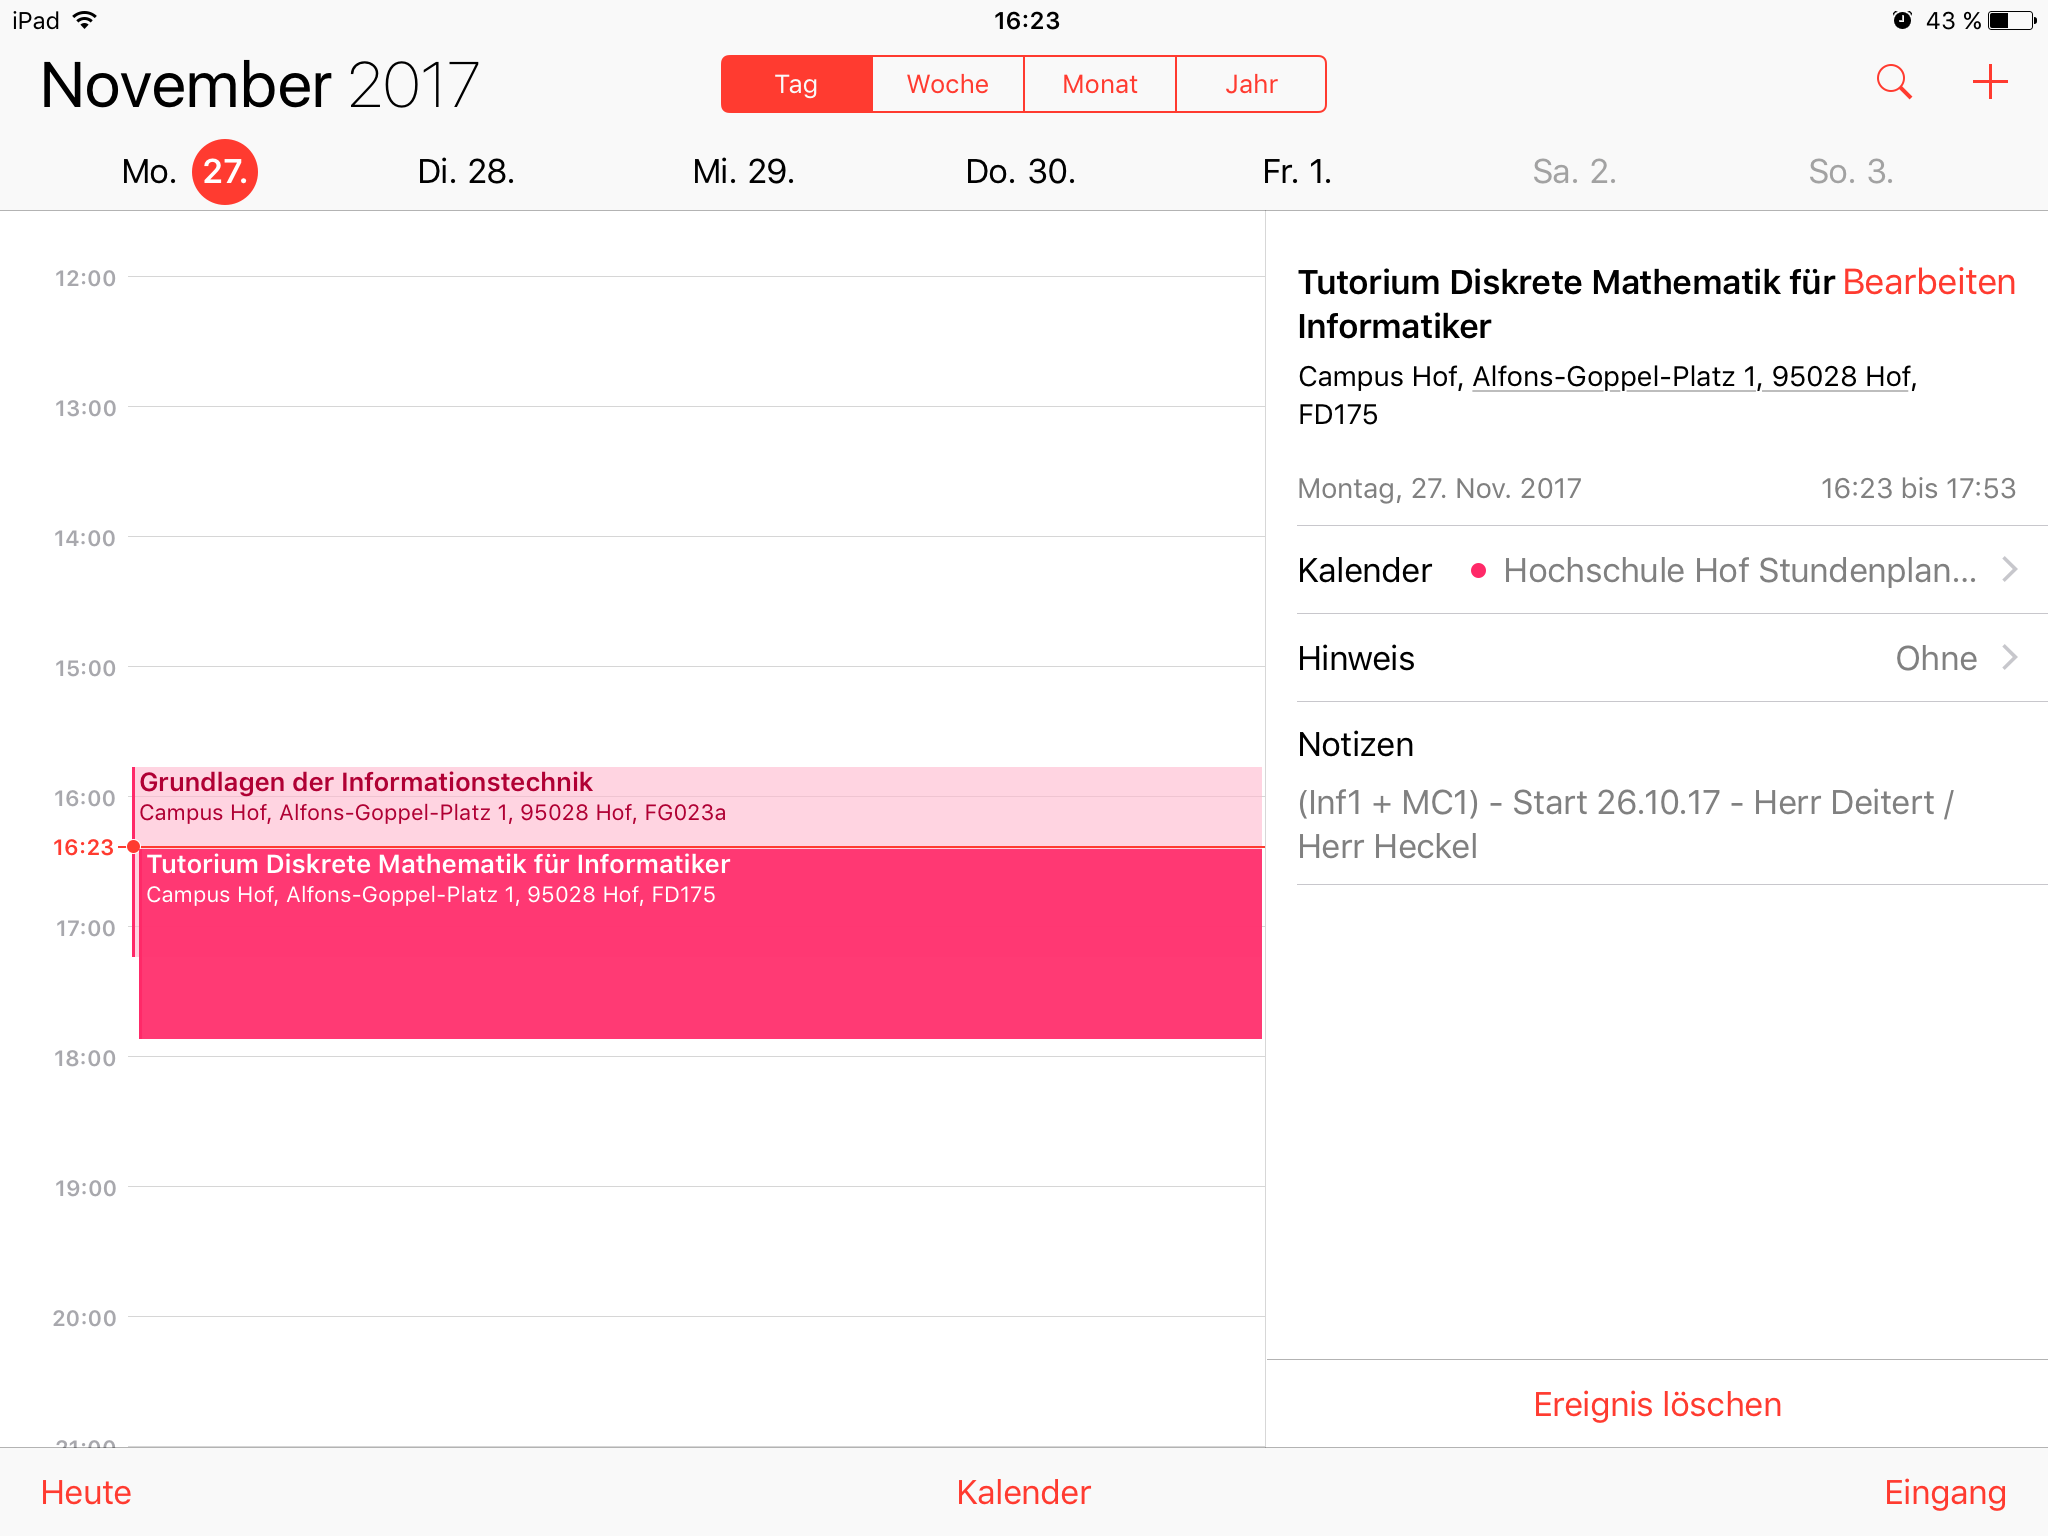
\includegraphics[scale=0.2]{test_vorlesung}}
	\caption{testingBug1}
	\label{fig1}
\end{figure}



\newpage
\section{Durchführung V3.2}
\subsection{Stundenplan}
Version 3.2 vom 01.12.2017 Testflight Version 4\newline
\noindent%
\begin{tabularx}{\textwidth}{|p{.55\textwidth}|X|X|X|X|X|X| }
\hline
\textbf{Studiengänge} &\textbf{Test 1} &\textbf{Test 2} &\textbf{Test 3}&\textbf{Test 4} &\textbf{Test 5} &\textbf{Test 6}  \\ \hline 

BBB  Berufsbegleitender Bachelor Betriebswirtschaft & X & X & X & X & X & X  \\ \hline
BBB I  Berufsbegleitender Bachelor Betriebswirtschaft SP Industrie- und Dienstleistungsunternehmen & X & X & X & X & X & X  \\ \hline
BW dual  Betriebswirtschaft dual & X & X & X & X & X & X  \\ \hline
Inf  Informatik & X & X & X & X & X & X  \\ \hline
Master GMA  Master General Management & X & X & X & X & X & X  \\ \hline
Master IP  Master Internationales Personalmanagement & X & X & X & X & X & X  \\ \hline
Master M  Master Marketing Management & X & X & X & X & X & X  \\ \hline
MD  Mediendesign & X & X & X & X & X & X  \\ \hline
MC  Mobile Computing & X & X & X & X & X & X  \\ \hline
Sprache  Sprachenprogramm & X & X & X & X & X & X  \\ \hline
UT  Umweltingenieurwesen & X & X & X & X & X & X  \\ \hline
Vinf  Verwaltungsinformatik & X & X & X & X & X & X  \\ \hline
WT  Werkstofftechnik & X & X & X & X & X & X  \\ \hline
Wing  Wirtschaftsingenieurwesen & X & X & X & X & X & X  \\ \hline
Wing PP Wirtschaftsingenieurwesen Produktion- und Prozessmanagement & X & X & X & X & X & X  \\ \hline
WR  Wirtschaftsrecht & X & X & X & X & X & X  \\ \hline
\end{tabularx}
 \newline
\newline

\noindent%
\begin{tabularx}{\textwidth}{|p{.2\textwidth}|X|X| }
\hline
\textbf{Studiengänge} &\textbf{Bemerkung / Auffäligkeiten}   \\ \hline 

BW dual  Betriebswirtschaft dual & 
Sem 3 Teilweise doppelte Einträge  \\ \hline

Sprache  Sprachenprogramm & 
Sprachauswahl Deutsch
Englisch Refresher Course nicht im Kalender am 13.12.2017 (ohne Spl-Änderungs-Angabe)
Türkisch Vorlesung und Änderung nur auf der Website; nicht in der VL Auswahl"   \\ \hline
Allgemein & Abbruch der Synchronisation beim ändern des Tabs 
Bei erneut Synchronisieren mit Kalender -$>$ erneutes Einfügen im Kalender 
Anlegen eines neuen Kalender nach sofort Beenden der App und erneut Sync
-$>$ Kalender manuell löschen"  \\ \hline
Allgemein & Vorlesungsfreie Zeiten werden nicht berücksichtigt  \\ \hline
\end{tabularx}
\newpage
\subsection{Aufgetretene Bugs}
Beim Testen wurde festgestellt das es Schwierigkeiten mit der Übertragung zum Kalender gibt. Vorlesungseinträge waren doppelt, einige Vorlesungsänderungen fehlten auch in der App. Die Vorlesungen wurden auch in den vorlesungsfreien Zeiten im Kalender angezeigt. \newline
 
\begin{figure}[H]
	\centering
  \frame{ 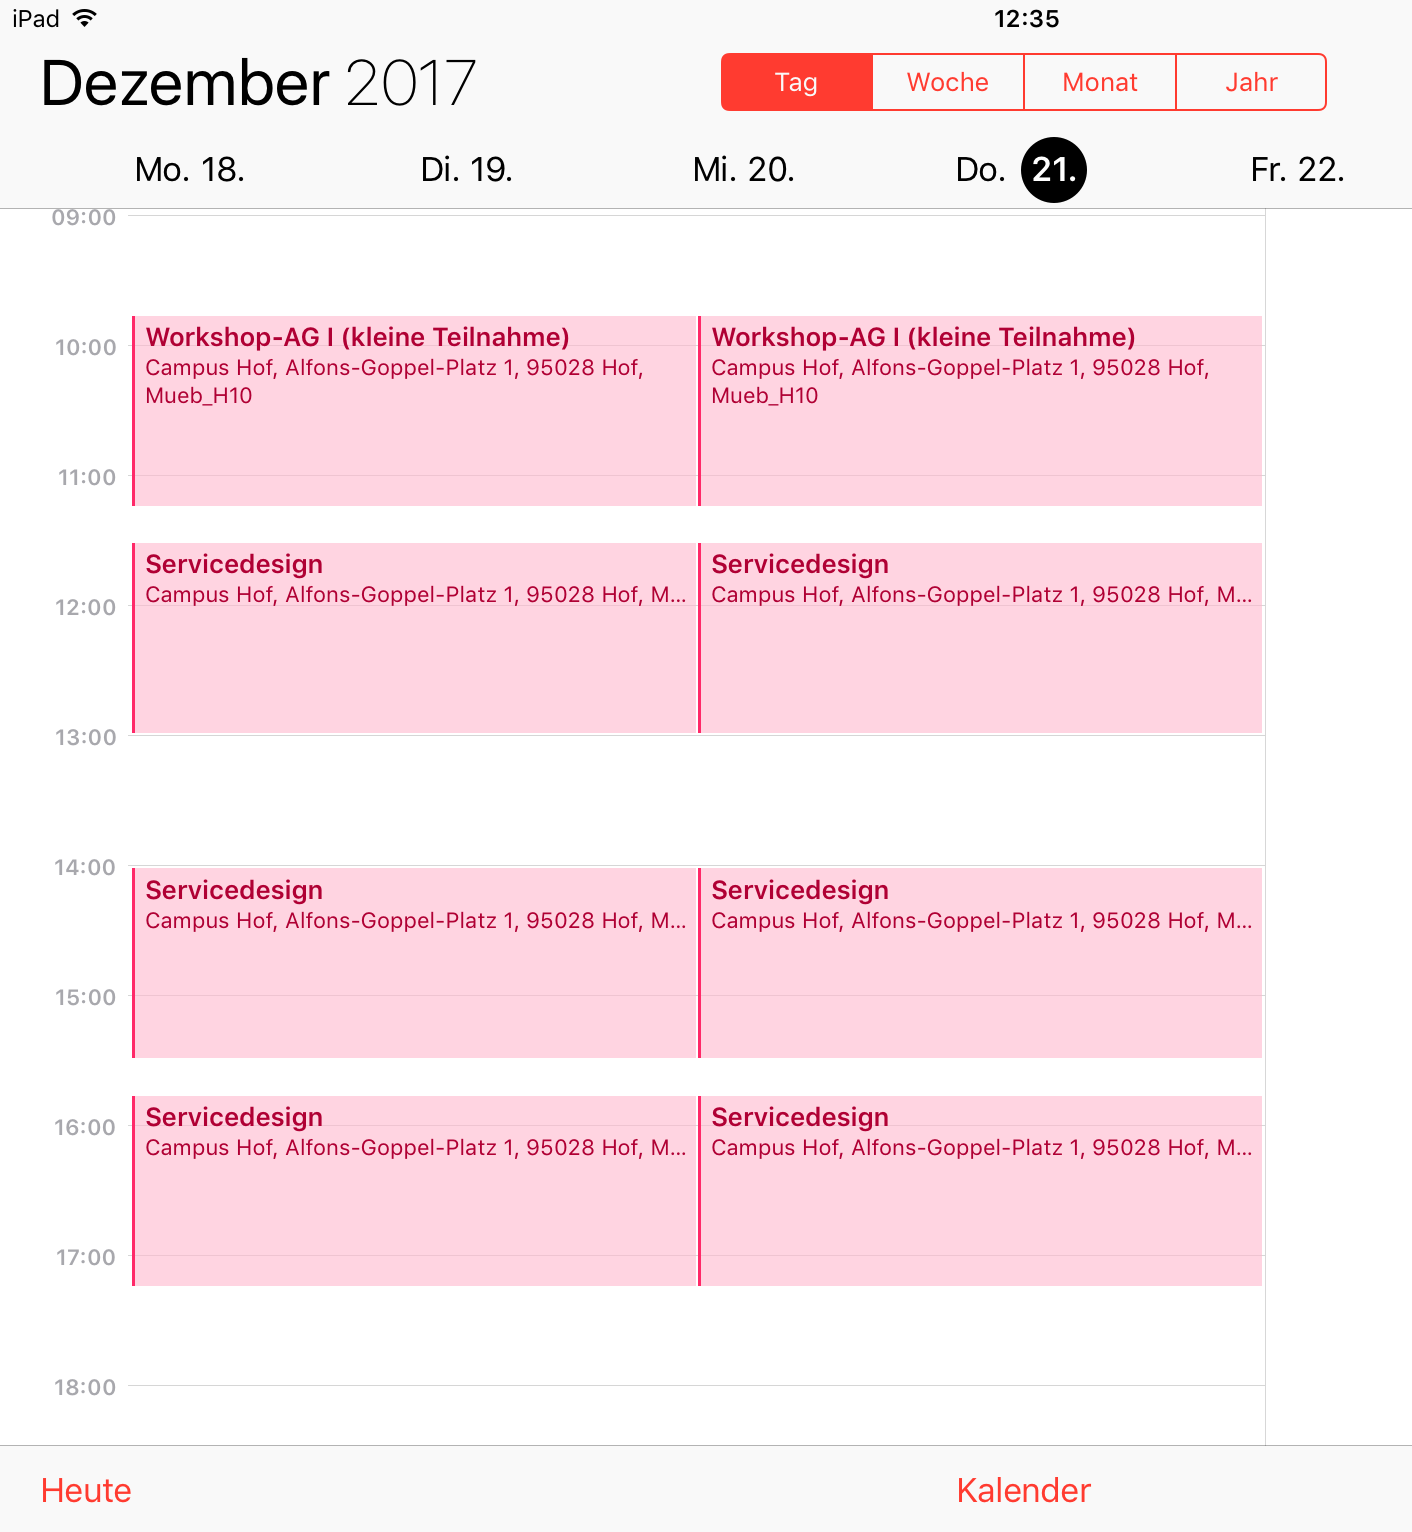
\includegraphics[scale=0.25]{test_doppelt}}
	\caption{testingBug2}
	\label{fig1}
\end{figure}

\section{Durchführung V4.0}
\subsection{Stundenplan}
Version 4.0 vom 19.01.2018\newline
\noindent%
\begin{tabularx}{\textwidth}{|p{.55\textwidth}|X|X|X|X|X|X| }
\hline
\textbf{Studiengänge} &\textbf{Test 1} &\textbf{Test 2} &\textbf{Test 3}&\textbf{Test 4} &\textbf{Test 5} &\textbf{Test 6}  \\ \hline 

BBB  Berufsbegleitender Bachelor Betriebswirtschaft & X & X & X & X & X &   \\ \hline
BBB I  Berufsbegleitender Bachelor Betriebswirtschaft SP Industrie- und Dienstleistungsunternehmen & X & X & X & X & X &   \\ \hline
BW dual  Betriebswirtschaft dual & X & X & X & X & X &  \\ \hline
Inf  Informatik & X & X & X & X & X &   \\ \hline
Master GMA  Master General Management & X & X & X & X & X &   \\ \hline
Master IP  Master Internationales Personalmanagement & X & X & X & X & X &  \\ \hline
Master M  Master Marketing Management & X & X & X & X & X &   \\ \hline
MD  Mediendesign & X & X & X & X & X &   \\ \hline
MC  Mobile Computing & X & X & X & X & X &  \\ \hline
Sprache  Sprachenprogramm & X & X & X & X & X &  \\ \hline
UT  Umweltingenieurwesen & X & X & X & X & X &   \\ \hline
Vinf  Verwaltungsinformatik & X & X & X & X & X &  \\ \hline
WT  Werkstofftechnik & X & X & X & X & X &  \\ \hline
Wing  Wirtschaftsingenieurwesen & X & X & X & X & X &  \\ \hline
Wing PP Wirtschaftsingenieurwesen Produktion- und Prozessmanagement & X & X & X & X & X &   \\ \hline
WR  Wirtschaftsrecht & X & X & X & X & X &  \\ \hline
\end{tabularx}
 \newline
\newline

\noindent%
\begin{tabularx}{\textwidth}{|p{.2\textwidth}|X|X| }
\hline
\textbf{Studiengänge} &\textbf{Bemerkung / Auffäligkeiten}   \\ \hline 

BBB  Berufsbegleitender Bachelor Betriebswirtschaft & 
Probleme mit Calender - Syncronisation
Kalender verschwindet bei Änderung des Semesters   \\ \hline  

BW dual  Betriebswirtschaft dual & 
Probleme mit Calender - Syncronisation
Kalender verschwindet bei Änderung des Semesters \\ \hline
 
Inf  Informatik & 
Sem 1 nur Tutoriums-Einträge
Sem 3 CalendarInterface-removeCalendar-error
Error Domain=EKErrorDomain Code=11 "That event does not belong to that event store." UserInfo={NSLocalizedDescription=That event does not belong to that event store.}   \\ \hline   
 
Sprache  Sprachenprogramm & 
Deutsch wurde in Kalender übernommen   \\ \hline   
 
WT  Werkstofftechnik & 
Sem 3: %202&id[]=GdM%C2%A7jbeck%2557224%20$%202&id[]= position : 0
2018-01-22 04:39:31.976725+0100 StundenplanNavigation[710:147415] [Warning] Warning once only: Detected a case where constraints ambiguously suggest a height of zero for a tableview cell's content view. We're considering the collapse unintentional and using standard height instead.
Jobposition kommt zurück in update: 0
Extract Changes
DataObserver wird benachrichtigt
Lade Daten für Changes neu (tableview update)
- true
ScheduleChanges Controller All Jobs Done
All NetworkJobs Canceled   \\ \hline
 
Wing PP  Wirtschaftsingenieurwesen Produktion- und Prozessmanagement & 
Sem 5 nur Freitagsvorlesung im Kalender   \\ \hline   
   
WR  Wirtschaftsrecht & 
Sem 1 nur Einführung in die Rechtswissenschaft Do / Fr / Sa
Sem 1b Kalender wurde nicht geladen:
Jobposition kommt zurück in update: 0
Extract Changes
füge element Wirtschaftsprivatrecht Grundlagen zu savedplusname hinzu
DataObserver wird benachrichtigt
Changes geladen
lecture not found
ScheduleChanges Controller All Jobs Done
Sem 3 Montag nur Rechtssicherung
Sem 5 bei Kalendersyncronisation:
StundenplanNavigation[741:159584] Error loading default properties for object x-apple-eventkit:///(null)/p93076 from daemon: Error Domain=EKCADErrorDomain Code=1010 "(null)"
lecture not found
lecture not found
lecture not found
lecture not found
lecture not found
lecture not found
lecture not found
Sem 5d:
CalendarInterface-removeCalendar-error
Error Domain=EKErrorDomain Code=11 "That event does not belong to that event store." UserInfo={NSLocalizedDescription=That event does not belong to that event store.}   \\ \hline

\end{tabularx}
\newpage

\subsection{Onboarding}
\noindent%
\begin{tabularx}{\textwidth}{|p{.75\textwidth}|X|X|X }
\hline
\textbf{Testschritte} &\textbf{Test 1} &\textbf{Test 2}  \\ \hline 

Onboarding starten -$>$ Farbe wählen -$>$ Studiengang wählen -$>$ Semester wählen -$>$ Fächer wählen -$>$ Notifications erlauben -$>$ mit Kalender Synchronisieren  durch die Screens navigieren & X &    \\ \hline

Onboarding von den Einstellungen starten &  & X   \\ \hline

\end{tabularx}
 \newline
\newline

\subsection{Funktion Aufgaben}

\noindent%
\begin{tabularx}{\textwidth}{|p{.04 \textwidth}|p{.84 \textwidth}|X|X|X| }
\hline
\textbf{Nr.} &\textbf{Testschritte} &\textbf{OK}   \\ \hline 
1 & Menü Aufgaben: Neue Aufgabe festlegen -$>$ Aufgabentitel festlegen -$>$ Datum eintragen -$>$ Vorlesung auswählen -$>$ Beschreibung eintragen -$>$ Speichern & X     \\ \hline
2 & Aufgaben Aktivieren/Deaktivieren -$>$ Sortieren nach Datum / Fach &     \\ \hline
\end{tabularx}
 \newline
  \newline

\noindent%
\begin{tabularx}{\textwidth}{|p{.1\textwidth}|X|X| }
\hline
\textbf{Test Nr.} &\textbf{Bemerkung / Auffäligkeiten}   \\ \hline 
1 & 
Beim Eintragen mehrzeiliger Beschreibung verscheindet im Querformat der eingegebene Text hinter der Tastatur. \\ \hline

 2 & 
Aufgabe wird nicht angezeigt
Aufgabe wird nach Neustart der App angezeigt
Aktiv - Deaktiv wird erst nach Umschalten des Tabs angezeigt 
Keine Anzeige in der Headerzeile  \\ \hline
\end{tabularx}
\newline
\newline

\subsection{Widget}
\noindent%
\begin{tabularx}{\textwidth}{|p{.04 \textwidth}|p{.84 \textwidth}|X|X|X| }
\hline
\textbf{Nr.} &\textbf{Testschritte} &\textbf{OK}   \\ \hline 
1 & Widget angezeigt Anzeige des Timers & X     \\ \hline
2 & Details anzeigen (Mehr/ Weniger anzeigen) & X    \\ \hline
3 & Zeitangabe Nächste Übernächste (bei Mehr anzeigen) & X   \\ \hline
4 & Zeitangabe Morgen Übermorgen (bei Mehr anzeigen) & X  \\ \hline
5 & Zeitangabe Datum (bei Mehr anzeigen) & X  \\ \hline
\end{tabularx}
\newline
\newline

\noindent%
\begin{tabularx}{\textwidth}{|p{.1\textwidth}|X|X| }
\hline
\textbf{Test Nr.} &\textbf{Bemerkung / Auffäligkeiten}   \\ \hline 
 1 & 
Widget nicht transparent im Simulator und iPad IOS 10.3  \\ \hline
Weiteres & 
Beim Klicken auf die Mitteilung keine Weiterleitung zur App  \\ \hline
\end{tabularx}
\newline
\newline

\subsection{Sonstige Tests}

\noindent%
\begin{tabularx}{\textwidth}{|p{.04 \textwidth}|p{.84 \textwidth}|X|X|X| }
\hline
\textbf{Nr.} &\textbf{Testschritte} &\textbf{OK}   \\ \hline 

1 & Benutzer hat die alte App (Version 3) auf dem Handy -$>$ installiert neue Version &      \\ \hline

\end{tabularx}
\newline
\subsection{Aufgetretene Bugs}
\begin{itemize}
\item Bei der Anwendung gab es Probleme mit der Kalendersynchronisation. Teilweise wurde der Kalender angelegt, ohne Vorlesungen im aktuellen Zeitraum, oder mit nur einer Vorlesung in der Woche.
\item Das Onboarding ließ sich einwandfrei Testen. Hier könnte noch eine Funktion zum Abbrechen eingebaut werden, wenn in den Einstellungen versehentlich auf den Button Onbording neustarten geklickt wurde.
\item Beim Anlegen von Aufgaben wird mehrzeiliger Aufgabentext von der Tastatur verdeckt. Bei der Anzeige von den Aufgaben wird der Text in der Headerzeile in der jeweiligen Sortierung nicht angezeigt.
\item Das Widget wird nicht transparent angezeigt, und die Weiterleitung nach dem Anklicken zur App könnte noch ergänzt werden.
\item Die sonstigen Tests konnten noch nicht durchgeführt werden, da die Version 4.0 noch nicht veröffentlicht wurde, und somit ein überinstallierten der vorherigen Version dieser App nicht testbar ist.
\end{itemize}
